\documentclass[english]{textolivre}

% metadata
\journalname{Texto Livre}
\thevolume{17}
%\thenumber{1} % old template
\theyear{2024}
\receiveddate{\DTMdisplaydate{2024}{5}{9}{-1}}
\accepteddate{\DTMdisplaydate{2024}{6}{3}{-1}}
\publisheddate{\DTMdisplaydate{2024}{10}{21}{-1}}
\corrauthor{Alain Presentación Muñoz}
\articledoi{10.1590/1983-3652.2024.52566}
%\articleid{NNNN} % if the article ID is not the last 5 numbers of its DOI, provide it using \articleid{} commmand 
% list of available sesscions in the journal: articles, dossier, reports, essays, reviews, interviews, editorial
\articlesessionname{articles}
\runningauthor{Sanz-Ramos et al.}
%\editorname{Leonardo Araújo} % old template
\sectioneditorname{Daniervelin Pereira}
\layouteditorname{João Mesquita}

\title{Video games are a useful didactic tool for learning history and mathematics: a systematic review}
\othertitle{Os videogames são uma ferramenta didática útil para a aprendizagem da história e da matemática: Uma revisão sistemática}

\author[1]{Sheila Sanz-Ramos~\orcid{0000-0003-4646-5543}\thanks{Email: \href{mailto:ssanzram@alumnos.unex.es}{ssanzram@alumnos.unex.es}}}
\author[2]{Alain Presentación-Muñoz~\orcid{0000-0002-5118-6779}\thanks{Email: \href{mailto:alain@unex.es}{alain@unex.es}}}
\author[3]{Alberto González-Fernández~\orcid{0000-0001-6277-9054}\thanks{Email: \href{mailto:albertogf@unex.es}{albertogf@unex.es}}}
\author[4]{Miguel Rodal~\orcid{0000-0003-1349-2203}\thanks{Email: \href{mailto:mrodal@unex.es}{mrodal@unex.es}}}
\author[2]{Jesús Acevedo-Borrega~\orcid{0000-0002-7234-8263}\thanks{Email: \href{mailto:jeacbo@unex.es}{jeacbo@unex.es}}}
\affil[1]{University of Extremadura, Faculty of Sports Science, Cáceres, Spain.}
\affil[2]{University of Extremadura, Faculty of Teaching Training, Education Sciences Department, Cáceres, Spain.}
\affil[3]{University of Extremadura, Faculty of Education and Psicology, Education Sciences Department. Cáceres, Spain.}
\affil[3]{University of Extremadura, Faculty of Sports Science, Bio\~{E}rgon Research Group, Cáceres, Spain.}

\addbibresource{article.bib}

\makeatletter
\newcommand\cref@smugglelabel{\let\cref@currentlabel\cref@gcurrentlabel@temp}
\newcommand\cref@updatelabeldata[1]{%
 \cref@constructprefix{#1}{\cref@result}%
  \@ifundefined{cref@#1@alias}%
    {\def\@tempa{#1}}%
    {\def\@tempa{\csname cref@#1@alias\endcsname}}%
  \protected@xdef\cref@gcurrentlabel@temp{%
    [\@tempa][\arabic{#1}][\cref@result]%
    \csname p@#1\endcsname\csname the#1\endcsname}%
  \aftergroup\cref@smugglelabel  
    }
% test if \@currentcounter is empty for unnumbered sections 
% see https://tex.stackexchange.com/questions/728247/again-on-longtable-vs-cleveref-incompatibility
\AddToHook{label}{\ifx\@currentcounter\@empty\else\cref@updatelabeldata{\@currentcounter}\fi} 

\begin{document}
\maketitle

\begin{polyabstract}
\begin{abstract}
Video games have always been an object of leisure and entertainment for children and adults. Ignorance has led many people to view these types of games in a negative, violent or addictive way. The objective of this systematic review was to determine the use of video games in the field of education, specifically in mathematics and history, and to identify the benefits of playing video games on students’ academic performance. Method: a search was carried out in different databases: Pubmed, Web of Science, SciELO and Scopus, including studies published up to March 2021. Results: video games in the historical field improve learning, historical academic performance and their approach to students as well as motivation, fun and engagement, history comprehension and acquisition; and in mathematics, improve academic performance and math learning, problem solving, entertainment, fun and enjoyment, as well as the commitment and involvement of students in mathematics. Conclusions: most of the studies show the usefulness of video games during the learning process of history and mathematics for children. The implementation of video games at school increases the academic performance of students and improves their motivation. Therefore, the incorporation of video games as an educational tool is recommended.

\keywords{Electronic games \sep Children \sep Education \sep Academic performance \sep Motivation}
\end{abstract}

\begin{portuguese}
\begin{abstract}
Os video games sempre foram um objeto de lazer e entretenimento para crianças e adultos. A ignorância tem levado muitas pessoas a encarar este tipo de jogos de forma negativa, violenta ou viciante. O objetivo desta revisão sistemática foi determinar a utilização de video games no domínio da educação, especificamente em matemática e história, e identificar os benefícios de jogar video games no desempenho acadêmico dos alunos. Método: foi efetuada uma pesquisa em diferentes bases de dados: Pubmed, Web of Science, SciELO e Scopus, incluindo estudos publicados até março de 2021. Resultados: os video games no domínio histórico melhoram a aprendizagem, o desempenho acadêmico histórico e a sua abordagem aos alunos, bem como a motivação, a diversão e o envolvimento, a compreensão e a aquisição da história; e em matemática, melhoram o desempenho acadêmico e a aprendizagem, a resolução de problemas, o entretenimento, a diversão e o prazer, bem como o empenho e o envolvimento dos alunos na matemática. Conclusões: a maioria dos estudos mostra a utilidade dos video games durante o processo de aprendizagem da história e da matemática para as crianças. A implementação de video games na escola aumenta o desempenho acadêmico dos alunos e melhora a sua motivação. Por conseguinte, recomenda-se a incorporação de video games como uma ferramenta educativa.

\keywords{Jogos eletrônicos \sep Crianças \sep Educação \sep Desempenho acadêmico \sep Motivação}
\end{abstract}
\end{portuguese}
\end{polyabstract}

\section{Introduction}
Video games, once considered purely recreational, are now recognized as powerful educational tools that enhance learning in subjects such as history and mathematics \cite{martinez_entertainment_2022}. Some studies observed that playing is crucial in children’s lives because it allows them to learn \cite{vygotsky_play_1967}. Playing from preschool age helps children to develop physically, mentally and socially \cite{groos_play_1901,bruner_juego_2003,liu_usability_2022}. Through play, children experience, imitate and relate themselves to the world around them. Moreover, knowledge is better acquired in a playful way while children have fun \cite{mora_juego_2016}. The game has evolved into a technological component that exists nowadays. Children and adolescents, who are increasingly immersed in the digital age, are more accustomed to the use of video games in their daily lives. Young people have replaced activities such as reading with video games. These types of actions have been exploited by educators for the so-called serious games. \textcite{michael_serious_2006} describe serious games as those whose main objective is to play and learn while the child is having fun, i.e. the game is given a formative and educational component.

Traditionally, video games have been linked to negative perceptions, including concerns about violence \cite{anderson_video_2000,gentile_effects_2004}, addiction \cite{salguero_measuring_2002,chiu_relative_2012}, and academic decline \cite{anand_study_2007,ip_gaming_2008}. \textcite{anderson_video_2000} demonstrated the correlation between violent video games and increased aggression over time. However, video games serve as valuable tools in various contexts. Critics often overlook their positive impact on physical activity, health, and education. Active video games, like exergames, promote physical activity, combatting sedentary lifestyles \cite{beltran-carrillo_videojuegos_2011,zhao_effects_2024}. They are also used in healthcare settings to alleviate the challenges faced by hospitalized children and adolescents \cite{ledo_rubio_videojuegos_2016,busto_martinez_uso_2012}. Additionally, video games aid in medical training, improving motor skills \cite{akand_does_2016}. They play a significant role in education, fostering creativity and enhancing problem-solving skills \cite{etxeberria_balerdi_videojuegos_2001,roncancio-ortiz_uso_2017,triberti_brain_2023}.

History was selected as one of the subjects for this review due to the prevalence of related video games and the observed benefits of incorporating historical content into education at various levels. For instance, \textcite{emmons_i_2021} exemplify the integration of history into university education through the use of When Rivers Were Trails. Similarly, video games have frequently been employed in mathematics education, with authors like \textcite{chorianopoulos_design_2014} developing serious video games tailored for mathematical learning. \textcite{drummond_video-games_2014} also highlight the positive impact of video games on mathematical academic performance. Despite these individual studies, there remains a gap in the literature regarding a comprehensive synthesis of the benefits of video games in both mathematics and history education. Therefore, this systematic review aims to address this gap by examining the utilization of video games in education, particularly in mathematics and history, and by elucidating the potential benefits for students’ academic performance and instructional applications.

\section{Methods}\label{sec-normas}
This systematic review was conducted following the statements and guidelines proposed in the Preferred Reporting Items for Systematic Reviews and Meta-Analyses Guidelines (PRISMA) \cite{moher_items_2014}.

Regarding the questions that this systematic review aims to answer, the first is to determine the use or application of video games in education, specifically in the subjects of history and mathematics. Another aspect to know is the benefits of the use of video games in the academic performance of both subjects and, finally, their possible applications in the educational field.


\subsection{Literature research}
The search was conducted up to March 2021 in the following electronic databases: PubMed (Medline), Web of Science, Scopus and SciELO. The terms used under different topics were: a) Method used (“esport”, “electronic sports”, “video games” and “strategy video games”), b) Implementation (“education”, “gamification” and “problem solving”) and c) Subjects in which they are implemented (“mathematics” and “history”). The search was carried out using the treatment and result variables, separated by the Boolean operator “AND”. The Boolean “OR” was also used to join the terms belonging to the same category.

In this case, the search was as follows: (“esport”, “electronic sports”, “video games” and “strategy video games”) AND (“education”, “gamification” and “problem solving”) AND (“mathematics” and “history”).

\subsection{Study selection and eligibility criteria}
Two evaluators, with experience in maths and history fields and university grades related to education, independently conducted the search and screening process. Possible disagreements were resolved through discussion or consultation with a third author. The inclusion criteria were as follows: a) original articles written in Spanish or English, b) participants aged between 6 and 18 years, and c) the interventions had to deal with the use of video games during mathematics or history teaching. The exclusion criteria were: a) articles were systematic reviews, books or conferences.

\subsection{Data collection and extraction}
The information included the following elements: participants/population, intervention, findings and outcomes (PICOS) following the recommendations of the PRISMA statement.

Different software, such as Microsoft Office Excel and Zotero, were used to process the data and organized the whole process.

The articles were divided into two tables: \Cref{tab01} includes all articles related to the subject of history. \Cref{tab02} includes all articles related to mathematics.

On the other hand, the third table includes all the benefits found in history and mathematics articles for possible application in education.

\subsection{Study selection}
Out of the initially identified 713 articles, 191 duplicates were removed, leaving 522 unique articles. After screening titles and abstracts, 162 articles were excluded as they were unrelated to the topic, resulting in 352 articles for full-text review. Following eligibility criteria, 6 articles were discarded for not being in English or Spanish, and 62 studies were excluded due to participants falling outside the age range of 6 to 18 years. Additionally, 150 articles were deemed irrelevant to the application of video games in history or mathematics. After excluding 91 articles such as systematic reviews, conferences, and books, a total of 51 articles were included in this systematic review. The PRISMA flow diagram is shown in \Cref{fig1}.

\begin{figure}
\centering
\begin{minipage}{.85\textwidth}
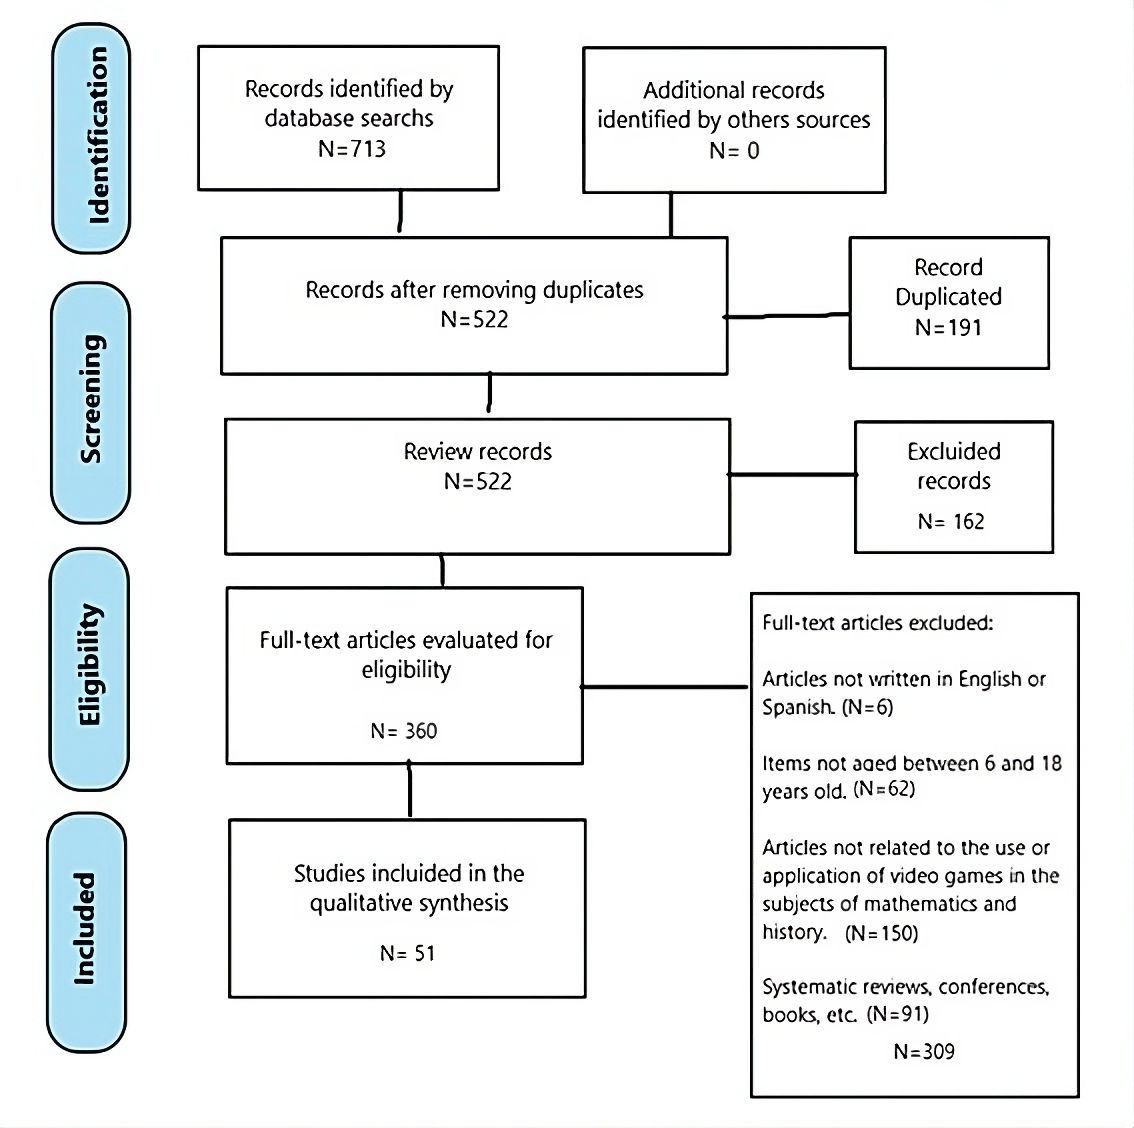
\includegraphics[width=0.85\linewidth]{Fig1_2.png}
\caption{Flow chart delineating the complete systematic review process.}
\label{fig1}
\source{Elaborated by the authors.}
\end{minipage}
\end{figure}

Subsequently, the articles were divided to determine all articles related to history or mathematics. These articles are analysed in the discussion section of this review and coincide with the questions posed in the Methods section and the Results tables: 37 articles correspond to the subject of mathematics and 14 articles belong to the subject of history.

\section{Results}\label{sec-conduta}
This section presents the results obtained from the systematic review of the selected studies. As indicated above, three tables can be found: \Cref{tab01} corresponds to studies or articles related to the use of video games in the subject of history, \Cref{tab02} is related to articles that use video games in the teaching of mathematics, and \Cref{tab03} lists the benefits of the use of video games in history and mathematics education.

\begin{footnotesize}
\begin{longtable}{
  >{\raggedright\arraybackslash}p{2cm}
  >{\raggedright\arraybackslash}p{2.2cm}
  >{\raggedright\arraybackslash}p{2.5cm}
  >{\raggedright\arraybackslash}p{3cm}
  >{\raggedright\arraybackslash}p{3cm}
}
\caption{Articles using video games for teaching history.}\label{tab01}
\\
\toprule
Citation & Participants & Intervention & Outcomes & Conclusions \\
\midrule
\textcite{bokolas_between_2019} & 5th and 6th grade students & Use of strategic video games once a week for 3 years. & The program made students learning more motivated and easier. & The video games used in the “history and video games” program helped the students to improve their knowledge of history. \\
\textcite{cornella_canals_design_2013} & 4th, 5th and 6th grade students and 1st and 2nd ESO students & A small satisfaction survey was conducted among beta-tester players. & The game was liked by 93\% of the players. They emphasize that it is fun, entertaining and promotes various skills. & \textit{Girona Legends} is a good method for learning history. \\
\textcite{evaristo_chiyong_uso_2016} & 561 secondary school students & Intervention in three study groups (1) with video games, (2) with history books and (3) with both. & The video game as a supplement had a greater effect on students’ grades. & Video games of this type could be used as a pedagogical tool in the teaching of History. \\
\textcite{gali_visiting_2019} & Secondary students & Evaluation of the gameplay of this serious game and, later, the motivation of the game in learning the story. & The game is attractive, has good gameplay and increases the interest of the students in the story. & Serious video games help motivation and the learning of history. \\
\textcite{gilbert__2019} & Secondary students & Qualitative interview study that uses \textit{Assassin’s Creed}, a narrative video game with a historical setting, as a site of inquiry. & There was a sense of immediate access to history contrasted with learning in school, a sense of human connection to people from the past, and a greater insight into multiple perspectives on history. & It is important to foster a sense of human connection to history through social education. \\
\textcite{jaldon-mendez_sanchez_uso_2021} & 1st ESO students & Using the \textit{Dominations} video game as a tool for learning history in the classroom. & \textit{Dominations} improve motivation in the classroom, the perception of content and the understanding of historical time. & Excellent tool within the formal educational framework for teaching and learning about the Mesopotamian civilization. \\
\textcite{martinez_soto_evaluacion_2018} & 34 students of 4th ESO & Evaluation-type research on a historically-themed virtual reality video game (28 items). & Positive general reception by the participants towards the contents of the video game as well as its value as a motivational element. & The video game brings students closer to living the experience in first person, making learning more immersive. \\
\textcite{Rea-Penafiel_2020} & 32 primary school students & Use of a video game for teaching history with mixed methods. & The video game demonstrated quality in consolidated percentage use in terms of effectiveness, efficiency, satisfaction, freedom from risk and context coverage. & This video game is effective for teaching history to elementary school students. \\
\textcite{ruth_commercial_2021} & 17 students from a 12th grade advanced history course & Video game study trade related to the history curriculum. & The students felt motivated towards historical content and addressed social issues. & Video games are a useful tool for teaching and learning history. \\
\textcite{saez-lopez_exploring_2015} & Secondary students & Use of \textit{MinecraftEdu} in a study in the field of history. & \textit{MinecraftEdu} is fun, encourages creativity, encourages discovery, and is a good app for creating and exploring immersive historical environments. & The use of \textit{MinecraftEdu} helps to motivate students in the field of history. \\
\textcite{jaldon-mendez_sanchez_uso_2021} & 1st ESO students & Using \textit{Dominations} to improve the acquisition of Mesopotamian historical knowledge. & Greater motivation in the classroom, a better perception of the content, as well as a better understanding of historical time. & \textit{Dominations} is an excellent tool within the formal educational framework for teaching and learning about the Mesopotamian civilization. \\
\textcite{sar_role_2012} & Children of 6th, 7th and 8th grade of primary school & Using non-educational, historically-themed computer games to gain insight into history. & Positive results of historical computer video games among primary school students. & This type of games can be applied in the primary classroom to learn history. \\
\textcite{watson_case_2011} & Secondary 2nd grade students & Using Making History, a World War II video game, for educational purposes. & The students were much more active and engaged. & Making History helps students to be more engaged and active in learning history. \\
\textcite{yu_exploration_2014} & 103 high school students & Study 2 classes, one that used computer games about history to learn and a control class. & Students with video games obtained greater motivation and improved their learning achievements. & The use of video games in history classes increases learning achievement and motivation. \\
\bottomrule
\source{Elaborated by the authors.}
\end{longtable}
\end{footnotesize}

Articles examining the use and application of video games in history have identified several features that support their educational benefits. These include improvements in academic performance and learning outcomes facilitated by the integration of various video games. Other important factors include increased student motivation and engagement with historical content, improved comprehension and the accessibility of historical material through video games. Furthermore, history video games have been shown to be effective in motivating, entertaining and engaging students, serving as both a source of enjoyment and educational value. This dual function underlines their potential as a valuable tool in history education.

\begin{footnotesize}
\begin{longtable}{
  >{\raggedright\arraybackslash}p{2cm}
  >{\raggedright\arraybackslash}p{2.2cm}
  >{\raggedright\arraybackslash}p{2.5cm}
  >{\raggedright\arraybackslash}p{3cm}
  >{\raggedright\arraybackslash}p{3cm}
}
\caption{Articles using video games for teaching mathematics.}\label{tab02}
\\
\toprule
Citation & Participants & Intervention & Outcomes & Conclusions \\
\midrule
\textcite{albarracin_secuencia_2021} & 78 4th grade students & \textit{Kula World} was used in 4 related activities. & Positive results in three-dimensional visualization and problem solving. & The video game and activities are useful for three-dimensional visualization. \\
\textcite{albarracin_taller_2019} & 24 students of 3rd ESO & Use of a strategy video game during 16 sessions. & Students boost their math skills and problem solving. & The video game helps with real math situations. \\
\textcite{alzahrani_evaluation_2013} & 20 students from 4th-5th grade of primary school & Use of a workshop with Microsoft’s \textit{Kodu} video game platform. The students evaluated the workshop as effective and entertaining. & Microsoft’s \textit{Kodu} platform helps to understand mathematical content. \\
\textcite{baig_effect_2020} & 789 4th, 5th and 6th grade students & 2 different treatments: traditional learning methods and a video game based on the Mathematics curriculum. & Video games based on the Mathematics curriculum had a positive effect on student performance. & Curriculum-based video games were more effective than traditional methods. \\
\textcite{barrios_matelogic:_2018} & 3rd grade students & Using \textit{Matelogic} with trial-error sessions on tangible programming. & Favorable results on the use of video games among students compared to traditional methods. & Algorithmic thinking concepts and video game interaction provide favorable learning outcomes, surpassing traditional methods. \\
\textcite{chen_design_2014} & Elementary students & Quasi-experimental method in urban and rural primary schools. & Digital game-based learning produced better learning effects. & Learning with video games is a good way to improve math learning compared to traditional learning. \\
\textcite{deater-deckard_student_2014} & 97 children from 11 to 14 years old Using a serious digital math game for the iPad. & Most of the students were highly engaged, attentive, and improved in math. & Commitment, attention and persistence can be improved through a video game. \\
\textcite{drigas_line_2015} & Primary, secondary and university students & Analysis of the effects of video games on students’ mathematical performance and cognitive skills. & Improve visual attention, cognitive skills, memory, comprehension and mathematical problem solving, motivation and few academic improvements. & Video games could be useful learning aids to build an innovative teaching model. \\
\textcite{ester_aprender_2022} & 279 students of 3rd and 4th grade of Primary Education & Use of mathematical video games as part of a regular training of one hour per week for 7 months. & The improvement was more significant in 3rd grade students than in 4th grade students. & Mathematics competence improved in those students with a longer exposure time to the intervention. \\
\textcite{del_moral_perez_game-based_2018} & 101 1st grade students & Case study aimed at verifying the possible increase in Multiple Intelligences among students with video games. & There was a general increase of all Multiple Intelligences. & The introduction of a video game in the classroom is suitable for Multiple Intelligences in primary school. \\
\textcite{fokides_digital_2018} & 201 1st, 4th and 6th grade students & Project with \textit{Kodu Lab Game} digital games for teaching Mathematics. & The students in the gaming group outperformed the students in the other groups in most cases. & Microsoft’s \textit{Kodu Lab Game} helps with learning mathematics and makes the user enjoy it. \\
\textcite{fraga-varela_impact_2021} & 284 students from first to fourth grade & Quasi-experimental study with several experimental groups to know the impact of serious video games in the mathematics classroom. & A significant improvement in mathematical fluency with the use of serious games in the different courses and classroom groups studied. & The use of serious video games designed specifically for school settings has the potential to teach mathematics. \\
\textcite{fraga-varela_impact_2021} & 284 students from first to fourth grade & Quasi-experimental study with several experimental groups to find out the impact of serious video games on mathematical fluency. & The software benefits boys and girls equally, and there is a clear relationship between the results obtained and the performance in the overall grades of the students. & It shows the potential of serious games in the school setting and the opportunity to address gender differences in performance. \\
\textcite{goldin_far_2014} & 6-year-old students & Analysis of computer games in executive functions versus traditional tests. & The intervention causes transfer to some (but not all) facets of executive function. & The intervention equalizes the academic results of children who regularly attend school. \\
\textcite{graziano_enhanced_1999} & 237 second graders & Using Spatia 1-\textit{Temporal Math} Video Game software designed to teach fractions and proportional math. & Children who received piano keyboard training along with math video game scored higher. & This approach can easily be used to teach other mathematical and scientific concepts in a complementary way to traditional methods. \\
\textcite{hanghoj_digital_2022} & 190 high school students (32 at risk) & 3-week intervention with game-based learning activities in eight lower secondary classrooms. & A positive impact on the well-being of at-risk students and reduced experiences of external regulation to engage in Mathematics. Game-based classrooms allow you to reframe social participation and student engagement with the curriculum, as well as their motivation. \\
\textcite{hieftje_evaluation_2017} & 134 first grade students & Open-label randomized controlled trial to determine the impact of the \textit{Knowledge Battle} video game on mathematics scores and self-competence. & \textit{Knowledge Battle} improved math skills in participants who played the game. & \textit{Knowledge Battle} was an acceptable and enjoyable educational math video game for first graders. \\
\textcite{holguin-alvarez_gamificacion_2022} & 300 third and fourth grade students & Educational platforms and video game competition for six months. & An increase in scores indicating improvements in the non-connective demand approach and in the connective demand approach. & The combinatorial effects of the use of technological resources to gamify are positive in the performance in the mathematical cognitive demand. \\
\textcite{holguin-alvarez_modificacion_2022} & 250 students & Six months of research development with the experimental model. & Better possibilities of producing mathematical operations based on reasoning were produced, provoking greater reflection in the experimental group. & It is necessary to deepen the evidence on the level of connective demand (high level) with other Latin American samples. \\
\textcite{holguin_alvarez_proyectos_2020} & 79 vulnerable students in the third and fourth grade of primary school & Educational projects with video games such as gamifiers basics to develop mathematical thinking. & There were positive results in reasoning and mathematical thinking. & The study contributed to the understanding of the gamification of educational projects as a companion in the didactics of mathematics. \\
\textcite{holguin-alvarez_gamificacion_2019} & 139 elementary students & Three stimulus experiments using \textit{Candy Crush, Asphalt 8 Airborne} and \textit{Plants vs Zombies}. & Lower rates of increase in scores in numeration, and higher in mathematical reasoning and problem solving. & The video games used improve mathematical reasoning and problem solving. \\
\textcite{hussain_digital_2017} & 39 students & Quasi-experimental study in a school using digital game-based learning in mathematics. & The use of digital game-based learning could increase the performance of students in the subject of Addition of less than 100. & Digital game-based learning can be used as an alternative reference strategy for the Mathematics teacher. \\
\textcite{karki_improving_2022} & 195 fifth and sixth grade students Quasi-experimental design of the \textit{NanoRoboMath} game to improve knowledge of adaptive and conceptual rational numbers. & A small positive effect of playing the \textit{NanoRoboMath} game on students’ conceptual knowledge of rational numbers was observed. & \textit{NanoRoboMath} is a useful video game for teaching adaptive and conceptual rational numbers. \\
\textcite{kebritchi_effects_2010} & 193 students & Experimental study playing a computer game to measure performance, motivation, and prior mathematical knowledge. & Significant improvement in the achievement of the experimental group compared to the control group and greater motivation. & Computer games are useful for improving mathematical knowledge, performance and motivation. \\
\textcite{kert_comparing_2017} & 105 fifth graders & Play a strategy game for the first time for 30 minutes to find out the correlation between academic performance and score. & Participants’ math or physical science skills were positively correlated with game success. & Strategy games help to positively improve mathematical academic performance. \\
\textcite{kiili_using_2015} & 66 students between 11 and 13 years old & Study on the use of \textit{Semideus} and \textit{Wuzzit Trouble} to work rational numbers and integer arithmetic, as well as the improvement of mathematical thinking and problem solving. & Games can be used to assess mathematical knowledge in a valid way, and brief interventions with these video games can be very effective. & The evaluation with video games is more effective than a simple measurement of precision and is more complete. \\
\textcite{kim_effects_2017} & 132 fourth graders & Performance test using a VR simulator for troubleshooting. & Significantly positive effect in the group with learning based on video games with virtual reality. & The use of a virtual reality simulator for problem solving is positive for the students. \\
\textcite{praveen_kumar_g._influence_2022} & 90 high school students Test after the use of educational video games for learning and retention in mathematics. & There was a significant difference in post-test scores between the experimental group and the control group. & Learning educational video games significantly improves students’ ability to achieve and retain. \\
\textcite{Li_2018} & Elementary students & Study on the use of \textit{See me Roar}, an augmented reality video game in mathematics, compared to traditional exercises. & Significantly improved the likeability, enjoyment, desire to do the exercise in spare time, and made math more fun. & \textit{See me Roar} makes it easier to do math homework positively versus traditional paper exercises. \\
\textcite{mangowal_mathbharata:_2017} & 85 school students with and without disabilities & Using \textit{MathBharata} to improve students’ motivation towards mathematics. & All students who tried \textit{MathBharata} increased their motivation towards mathematics. & \textit{MathBharata} is a useful tool to engage and motivate students towards mathematics. \\
\textcite{medina_camacho_harnessing_2022} & 5th grade students & Mixed research on the use of a video game (\textit{Kodu}) for logical-mathematical skills for 3 years. & Significant progress in the results obtained during the three years. & \textit{Kodu} improves students’ logical-mathematical skills and STEAM competition skills. \\
\textcite{nunes_liber_2022} & 6th graders & Using \textit{Liber Domus}, a video game to learn, understand and retain math concepts. & The game helps students to have a more dynamic approach in the classroom, increases motivation and allows flexibility and less repetition in revision. & \textit{Liber Domus} is useful for students’ learning, understanding, motivating and retaining mathematical concepts. \\
\textcite{pires_building_2019} & 64 first graders & Intervention of 13 days divided into virtual interaction (mathematical video game), tangible interaction and control group. & The virtual interaction group obtained higher performance and a significant improvement in mathematics. & The use of video games for teaching mathematics improves performance. \\
\textcite{pradiante_contribution_2022} & 12 children, 9 with ASD and 3 with Dyscalculia & Study of 12 sessions (1 session of 45 minutes per week) using a video game on mathematics and dyscalculia. & The children were motivated, participatory, and committed to learning mathematics. & The use of video games in the classroom helps children with Autism Spectrum Disorder (ASD) and dyscalculia when it comes to learning mathematics. \\
\textcite{walkington_effect_2022} & 85 secondary students & Assessment Conjectures geometric and cognitive relevance through the use of a video game. & Cognitive relevance influenced mathematical performance, as measured by the accuracy of students’ insights, knowledge, and demonstrations. & The use of a video game is useful for performance improvement and academic and cognitive relevance. \\
\textcite{wisittanawat_tricky_2021} & 2 high school students & Case analysis of 1 student who likes mathematics and 1 student who does not. They both use a math video game. & Both students were involved in the game and got great results. & Video games can make math classrooms more engaging for students. \\
\textcite{yong_let_2021} & 182 students & Use of computer video games on mathematics versus traditional teaching. & Students learn the process and receive feedback as they play computer games, as opposed to traditional teaching, which focuses on exams. & Mathematics-focused computer video games help grasp the process of learning and understanding mathematics. \\
\bottomrule
\source{Elaborated by the authors.}
\end{longtable}
\end{footnotesize}

Regarding the articles that examine the use and application of video games in mathematics education, several aspects have been identified that support the effectiveness of video games as learning tools in this area. The integration of video games has been associated with increases, improvements and achievements in mathematical academic performance and learning, as well as increased student engagement. In addition, video games applied to mathematics have been found to promote student motivation, enjoyment and entertainment. These findings demonstrate that the use of video games in education, particularly in mathematics, is a beneficial tool for teaching and learning (\Cref{tab03}).

\begin{table}[h!]
\centering
\begin{threeparttable}
\caption{Benefits of using video games in education.}
\label{tab03}
\begin{tabular}{l}
\toprule
Benefits of using video games in historical and mathematics education \\
\midrule
Feedback \\
Problem solving \\
Fun \\
Motivation \\
Improved academic performance \\
Active students \\
Implication \\
\bottomrule
\end{tabular}
\source{Elaborated by the authors.}
\end{threeparttable}
\end{table}


\section{Discussion}\label{sec-fmt-manuscrito}
This systematic review focuses on the use and application of video games for both subjects. As noted above, a division has been made between articles dealing with video games in the subjects of history and mathematics. Finally, there is a section dealing with the benefits of video games in both subjects.

Some limitations of the study were the number of databases used, which is limited; the inclusion and exclusion criteria, which to some extent limit the search and exclude other studies that may provide interesting results; and the experience of the lead author, who had not previously conducted a systematic literature review.

In the future, this systematic review can be used as a reference for the design of educational practices, educational projects, or interventions in educational centres. It gathers a multitude of experiences with different video games, many of which are open access, to work on history and mathematics outside of traditional methodology.

\subsection{The use and application of video games in the subject of history}

Articles related to the use and application of video games in the subject of history revealed different characteristics that support their use in education. Among these aspects, we found improvements in academic performance and learning through the use of different video games \cite{sar_role_2012,cornella_canals_design_2013,yu_exploration_2014,saez-lopez_exploring_2015,evaristo_chiyong_uso_2016,bokolas_between_2019,Rea-Penafiel_2020,jaldon-mendez_sanchez_uso_2021}. Other important aspects are the motivation and engagement of students in history \cite{watson_case_2011,yu_exploration_2014,martinez_soto_evaluacion_2018,bokolas_between_2019,gali_visiting_2019,Rea-Penafiel_2020,jaldon-mendez_sanchez_uso_2021,ruth_commercial_2021} and the understanding of it \cite{gali_visiting_2019,Rea-Penafiel_2020,ruth_commercial_2021,jaldon-mendez_sanchez_uso_2021}, or the easy access to history that video games grant students \cite{gilbert__2019,ruth_commercial_2021}. It has also been shown that history video games are useful in motivating, amusing and entertaining students while teaching \cite{cornella_canals_design_2013,saez-lopez_exploring_2015}, making them a source of entertainment and learning, which makes them a beneficial tool for teaching history.

\subsection{The use and application of video games in the subject of mathematics}
Regarding the articles that use and apply video games in the subject of mathematics, different aspects were found that support the use of video games as learning methods in the field of mathematics education. An increase, improvement and achievement in terms of mathematical academic performance and mathematics learning was observed when using video games \cite{graziano_enhanced_1999,kebritchi_effects_2010,chen_design_2014,deater-deckard_student_2014,goldin_far_2014,drigas_line_2015,kiili_using_2015,hieftje_evaluation_2017,hussain_digital_2017,kert_comparing_2017,kim_effects_2017,barrios_matelogic:_2018,del_moral_perez_game-based_2018,fokides_digital_2018,albarracin_secuencia_2021,holguin-alvarez_gamificacion_2019,pires_building_2019,baig_effect_2020,albarracin_taller_2019,fraga-varela_impact_2021,yong_let_2021,ester_aprender_2022,holguin-alvarez_gamificacion_2022,holguin-alvarez_modificacion_2022,karki_improving_2022,medina_camacho_harnessing_2022,praveen_kumar_g._influence_2022,walkington_effect_2022}, as well as student engagement \cite{deater-deckard_student_2014,wisittanawat_tricky_2021,hanghoj_digital_2022,pradiante_contribution_2022}, and problem solving \cite{drigas_line_2015,albarracin_secuencia_2021,holguin-alvarez_gamificacion_2019}. Finally, it was also observed that video games applied to the subject of mathematics help students’ motivation, fun and entertainment \cite{alzahrani_evaluation_2013,drigas_line_2015,mangowal_mathbharata:_2017,Li_2018,nunes_liber_2022,pradiante_contribution_2022}. These aspects demonstrate that the use and application of video games in education, specifically in mathematics, is a beneficial tool for teaching and learning.

\subsection{Benefits of using video games in history and mathematics}
After analyzing all the previous articles, different benefits have been observed to be brought by the use and application of video games to the education of history and mathematics. Some of these benefits are motivation, entertainment or fun \cite{alzahrani_evaluation_2013,cornella_canals_design_2013,drigas_line_2015,saez-lopez_exploring_2015,mangowal_mathbharata:_2017,Li_2018,nunes_liber_2022,pradiante_contribution_2022}, feedback \cite{yong_let_2021}, problem solving \cite{drigas_line_2015,albarracin_taller_2019,holguin-alvarez_gamificacion_2019,albarracin_secuencia_2021}, improvement in academic performance \cite{graziano_enhanced_1999,kebritchi_effects_2010,sar_role_2012,cornella_canals_design_2013,chen_design_2014,deater-deckard_student_2014,goldin_far_2014,yu_exploration_2014,drigas_line_2015,saez-lopez_exploring_2015,evaristo_chiyong_uso_2016,hieftje_evaluation_2017,hussain_digital_2017,kert_comparing_2017,barrios_matelogic:_2018,del_moral_perez_game-based_2018,fokides_digital_2018,albarracin_taller_2019,bokolas_between_2019,holguin-alvarez_gamificacion_2019,pires_building_2019,baig_effect_2020,Rea-Penafiel_2020,albarracin_secuencia_2021,fraga-varela_impact_2021,jaldon-mendez_sanchez_uso_2021,yong_let_2021,ester_aprender_2022,holguin-alvarez_gamificacion_2022,holguin-alvarez_modificacion_2022,karki_improving_2022,walkington_effect_2022} and student involvement and commitment \cite{watson_case_2011,deater-deckard_student_2014,yu_exploration_2014,martinez_soto_evaluacion_2018,bokolas_between_2019,gali_visiting_2019,Rea-Penafiel_2020,jaldon-mendez_sanchez_uso_2021,ruth_commercial_2021,wisittanawat_tricky_2021,hanghoj_digital_2022,pradiante_contribution_2022}.


\section{Conclusions}\label{sec-formato}
After conducting this systematic review, it is concluded that video games serve as valuable educational assets, particularly in mathematics and history. Analysis of the literature indicates that video games enhance learning, academic performance, and student engagement in historical studies. Similarly, their integration into mathematics education fosters improved acquisition of mathematical concepts, problem-solving skills, and student motivation. Moreover, video games facilitate enjoyable learning experiences and foster student commitment and participation in both subjects. Overall, the findings highlight the significant benefits of incorporating video games into classroom instruction.


\printbibliography\label{sec-bib}
%conceptualization,datacuration,formalanalysis,funding,investigation,methodology,projadm,resources,software,supervision,validation,visualization,writing,review
\begin{contributors}[sec-contributors]
\authorcontribution{Sheila Sanz-Ramosa}[conceptualization,review]
\authorcontribution{Alain Presentación-Muñoz}[conceptualization,writing]
\authorcontribution{Alberto González-Fernández}[investigation]
\authorcontribution{Miguel Rodal}[datacuration]
\authorcontribution{Jesús Acevedo-Borrega}[methodology]
\end{contributors}

\appendix

\section{Supplementary materials}

\begin{table}[h!]
\centering
\begin{threeparttable}
\caption{Supplementary materials}
\label{annex-tab01}
\begin{tabular}{p{3cm} p{10cm}}
\toprule
\multicolumn{2}{c}{Search Estrategy} \\
\midrule
Data base & Boolean vector \\
Web of Science & TI=((esport OR “electronic sports” OR “video games” OR “strategy video games”) AND (education OR gamification OR “problem solving”) AND (mathematics OR history)) OR AB=((esport OR “electronic sports” OR “video games” OR “strategy video games”) AND (education OR gamification OR “problem solving”) AND (mathematics OR history)) OR AK=((esport OR “electronic sports” OR “video games” OR “strategy video games”) AND (education OR gamification OR “problem solving”) AND (mathematics OR history)) \\
Scopus & TITLE-ABS-KEY ( ( esport OR “electronic sports” OR “video games” OR “strategy video games” ) AND ( education OR gamification OR “problem solving” ) AND ( mathematics OR history ) ) \\
SciELO & (“esport” OR “electronic sports” OR “video games” OR “strategy video games”) AND (education OR gamification OR “problem solving”) AND (mathematics OR history) \\
PubMed (Medline) & ((esport[TIAB] OR “electronic sports”[TIAB] OR “video games”[TIAB] OR “strategy video games”[TIAB]) AND (education[TIAB] OR gamification[TIAB] OR “problem solving”[TIAB]) AND (mathematics[TIAB] OR history[TIAB])) OR ((esport[MH] OR “electronic sports”[MH] OR “video games”[MH] OR “strategy video games”[MH]) AND (education[MH] OR gamification[MH] OR “problem solving”[MH]) AND (mathematics[MH] OR history[MH])) \\
\bottomrule
\end{tabular}
\source{Elaborated by the authors.}
\end{threeparttable}
\end{table}

\end{document}
